%\documentclass[12pt,preprint]{aastex6}
\documentclass[12pt]{article}

\bibliographystyle{aasjournal}

\usepackage{aas_macros} % need this because not using aastex or emulateapj
\usepackage{graphicx}
\usepackage[suffix=]{epstopdf}
\usepackage{natbib}
\usepackage{amsmath}
%\usepackage{url}
\usepackage{xspace}
\usepackage{fullpage}

%    Make Scientific Notation
\providecommand{\e}[1]{\ensuremath{\times 10^{#1}}}

% make the word Kepler italicized
\newcommand{\Kepler}{\textsl{Kepler}\xspace}
\newcommand{\racomment}[1]{{\color{red}#1}}
\newcommand{\ktwosc}{{\tt K2SC}}
\newcommand{\ktwo}{{\tt K2}}

% fuzzy math
\def\lesssim{\mathrel{\hbox{\rlap{\hbox{\lower3pt\hbox{$\sim$}}}\hbox{\raise2pt\hbox{$<$}}}}}
\def\gtrsim{\mathrel{\hbox{\rlap{\hbox{\lower3pt\hbox{$\sim$}}}\hbox{\raise2pt\hbox{$>$}}}}}

\begin{document}
%%%%%%%%%%%%%%%%%%%%%%

%Measuring Stellar Rotation with K2

\title{\vspace{-0.5in}Scientific/Technical/Management}
\date{}

\maketitle


% shrink up the space between the "title" and first section heading
\vspace{-1in}

%%%%%%%%%%%%%%%%%%%
\section{Introduction}

%% uhoh, i was about to send up an entire introduction... maybe we should coordinate more about writing sections! :)


Among the key observational properties of main sequence stars in our galaxy, age is the most difficult to determine. Traditionally, fitting isochrones to cluster stars was one of the only precise methods for measuring ages, and was impossible for the majority of isolated field stars. Methods such as asteroseismology and measuring Li abundances require time intensive observations for each target and are not capable of producing the large quantity of ages needed for exoplanet and galactic population studies. To improve our understanding of star and planet formation and evolution, as well as the history of the Milky Way, we must be able to constrain the ages of low-mass stars like the Sun in the galactic field.

Fortunately nature has provided a power means to determine ages for main sequence stars via their rotation. Angular momentum is carried away though magnetically driven stellar winds, which slows the star's rotation over cosmic time. This rotation-based ``clock'' is known as {\it gyrochronology}. Cool spots on the star's surface rotate in-to and out-of view, creating small amplitude ($\sim$1\%) quasi-periodic changes in the stellar brightness. While rotation periods have previously been laboriously measured from starspot-induced flux modulations for hundreds of stars, space-based photometric surveys have opened the door to homogeneous ensemble measures of stellar rotation, and therefore age.
{\bf With the precise, long-duration light curves available from the \Kepler/K2 mission, we can determine the rotation periods and ages for nearly 100,000 main sequence field stars.}
%Stellar rotation periods are are the most promising tool for constraining the ages of field stars.

The \Kepler mission broke new ground by producing rotation periods for tens-of-thousands of field stars within a single $\sim$110 sq deg field of view, and discovered a surprising bimodal distribution of rotation periods. Two competing explanations have arisen for this mysterious feature: a bimodal age distribution for nearby stars, or a new subtlety in stellar angular-momentum-loss mechanisms. Detailed calibrations of gyrochronology models with the \Kepler rotation sample also revealed the need for samples of stars with a wider range of ages and compositions. Fortunately the ongoing \Kepler extended mission, K2, has currently produced light curves from 14 additional fields throughout the Galaxy.

To enable studies of stellar ages from rotation periods with K2, we propose to:

{\bf 1.} Measure accurate rotation periods for every available K2 target, using new statistical methods we have developed to cope with significant instrumental systematics in the K2 data. This value-added dataset will improve the \Kepler data legacy for field stars, and provide a critical training set for the TESS mission.

{\bf 2.} Produce updated gyrochronology relations based on a wider range of field star ages, and additional open clusters within the K2 fields.

{\bf 3.} Determine the origin of the mysterious rotation period bimodality discoverd with \Kepler by tracing the rotation period distribution in each K2 field, and out to further distances utilizing public Gaia data.

{\bf 4.} Measure the star formation history within each K2 field using a new Bayesian age-dating system.



\clearpage



%%%%%%%%%%%%%%%%%%%
\section{Scientific Motivation}
Galactic archaeology and exoplanet populations are two rapidly accelerating
fields of interest within astronomy.
Although seemingly unconnected, these two fields are linked by a mutual
requirement for precise stellar parameters.
To galactic archaeologists, ages and elemental abundances are the most
important parameters.
Indeed, most galactic archaeology surveys target exactly these properties.
For exoplaneteers, masses and radii have historically been the most important
stellar parameters for understanding planetary systems. With a
growing number of planet hosts with precise masses and radii, attention is turning
toward other parameters such as ages to under the history and evolution of these systems.
Age is therefore a fundamental stellar parameter of great interest to two large
communities of astronomers. However it is a difficult attribute to measure for
main sequence F, G, K, and M stars in the field, in part because low-mass dwarfs do not move far on the Color-Magnitude
diagram (CMD) during their hydrogen burning lifetimes. Further,
competing stellar evolution models predict different ages for the same star.
%Asteroseismology, while a very precise age-dating tool, is not capable of
%producing the large quantity of ages needed for exoplanet and galactic
%population studies.
Of all the measurable properties for a large numbers of stars, rotation periods contain
the most information about stellar age, and provide the best leverage for advancing our knowledge of galactic archeology as well as exoplanet population demographics.




%%%%%%%%%
\subsection{Age-Dating Field Stars with Rotation}
The seminal work of \citet{skumanich1972} laid the foundation for our model of the stellar age--rotation--activity relationship. When stars settle onto the main sequence they may have a range of initial rotation periods based on the angular momentum available in their primordial environment. However, rotation velocities converge by a few 100 Myr (for Solar-type stars), and then follow a standard spin-down evolution \citep{barnes2010}. Stars continuously lose angular momentum due to magnetically driven winds. Stellar rotation also drives the internal magnetic dynamo, resulting in decreasing surface magnetic activity as the star slows (rotation period increases). Older, slower rotating stars therefore have smaller starspots, making the detection rotation more difficult as stars age. Deriving ages for field stars therefore requires knowing their color (as a proxy for stellar temperature or mass) and their surface rotation period \citep{barnes2007}, and can produce ages with errors as low as $\sim$10\% \citep{barnes2010}.

The rate of this angular momentum loss has historically been calibrated using main sequence stars at a range of masses in stellar clusters with known ages, leading to a useful clock called ``gyrochronology'' \citep{barnes2003}. Several gyrochronology model (or gyrochrones) parameterizations exist, each using various age benchmarks for calibration. Nearly all gyrochronology models suffer from lack of constraint at older ages; often the Sun is the only benchmark used older than $\sim$1 Gyr since accessible nearby open clusters are typically young ($<600$ Myr).

\begin{figure}[!t]
\centering
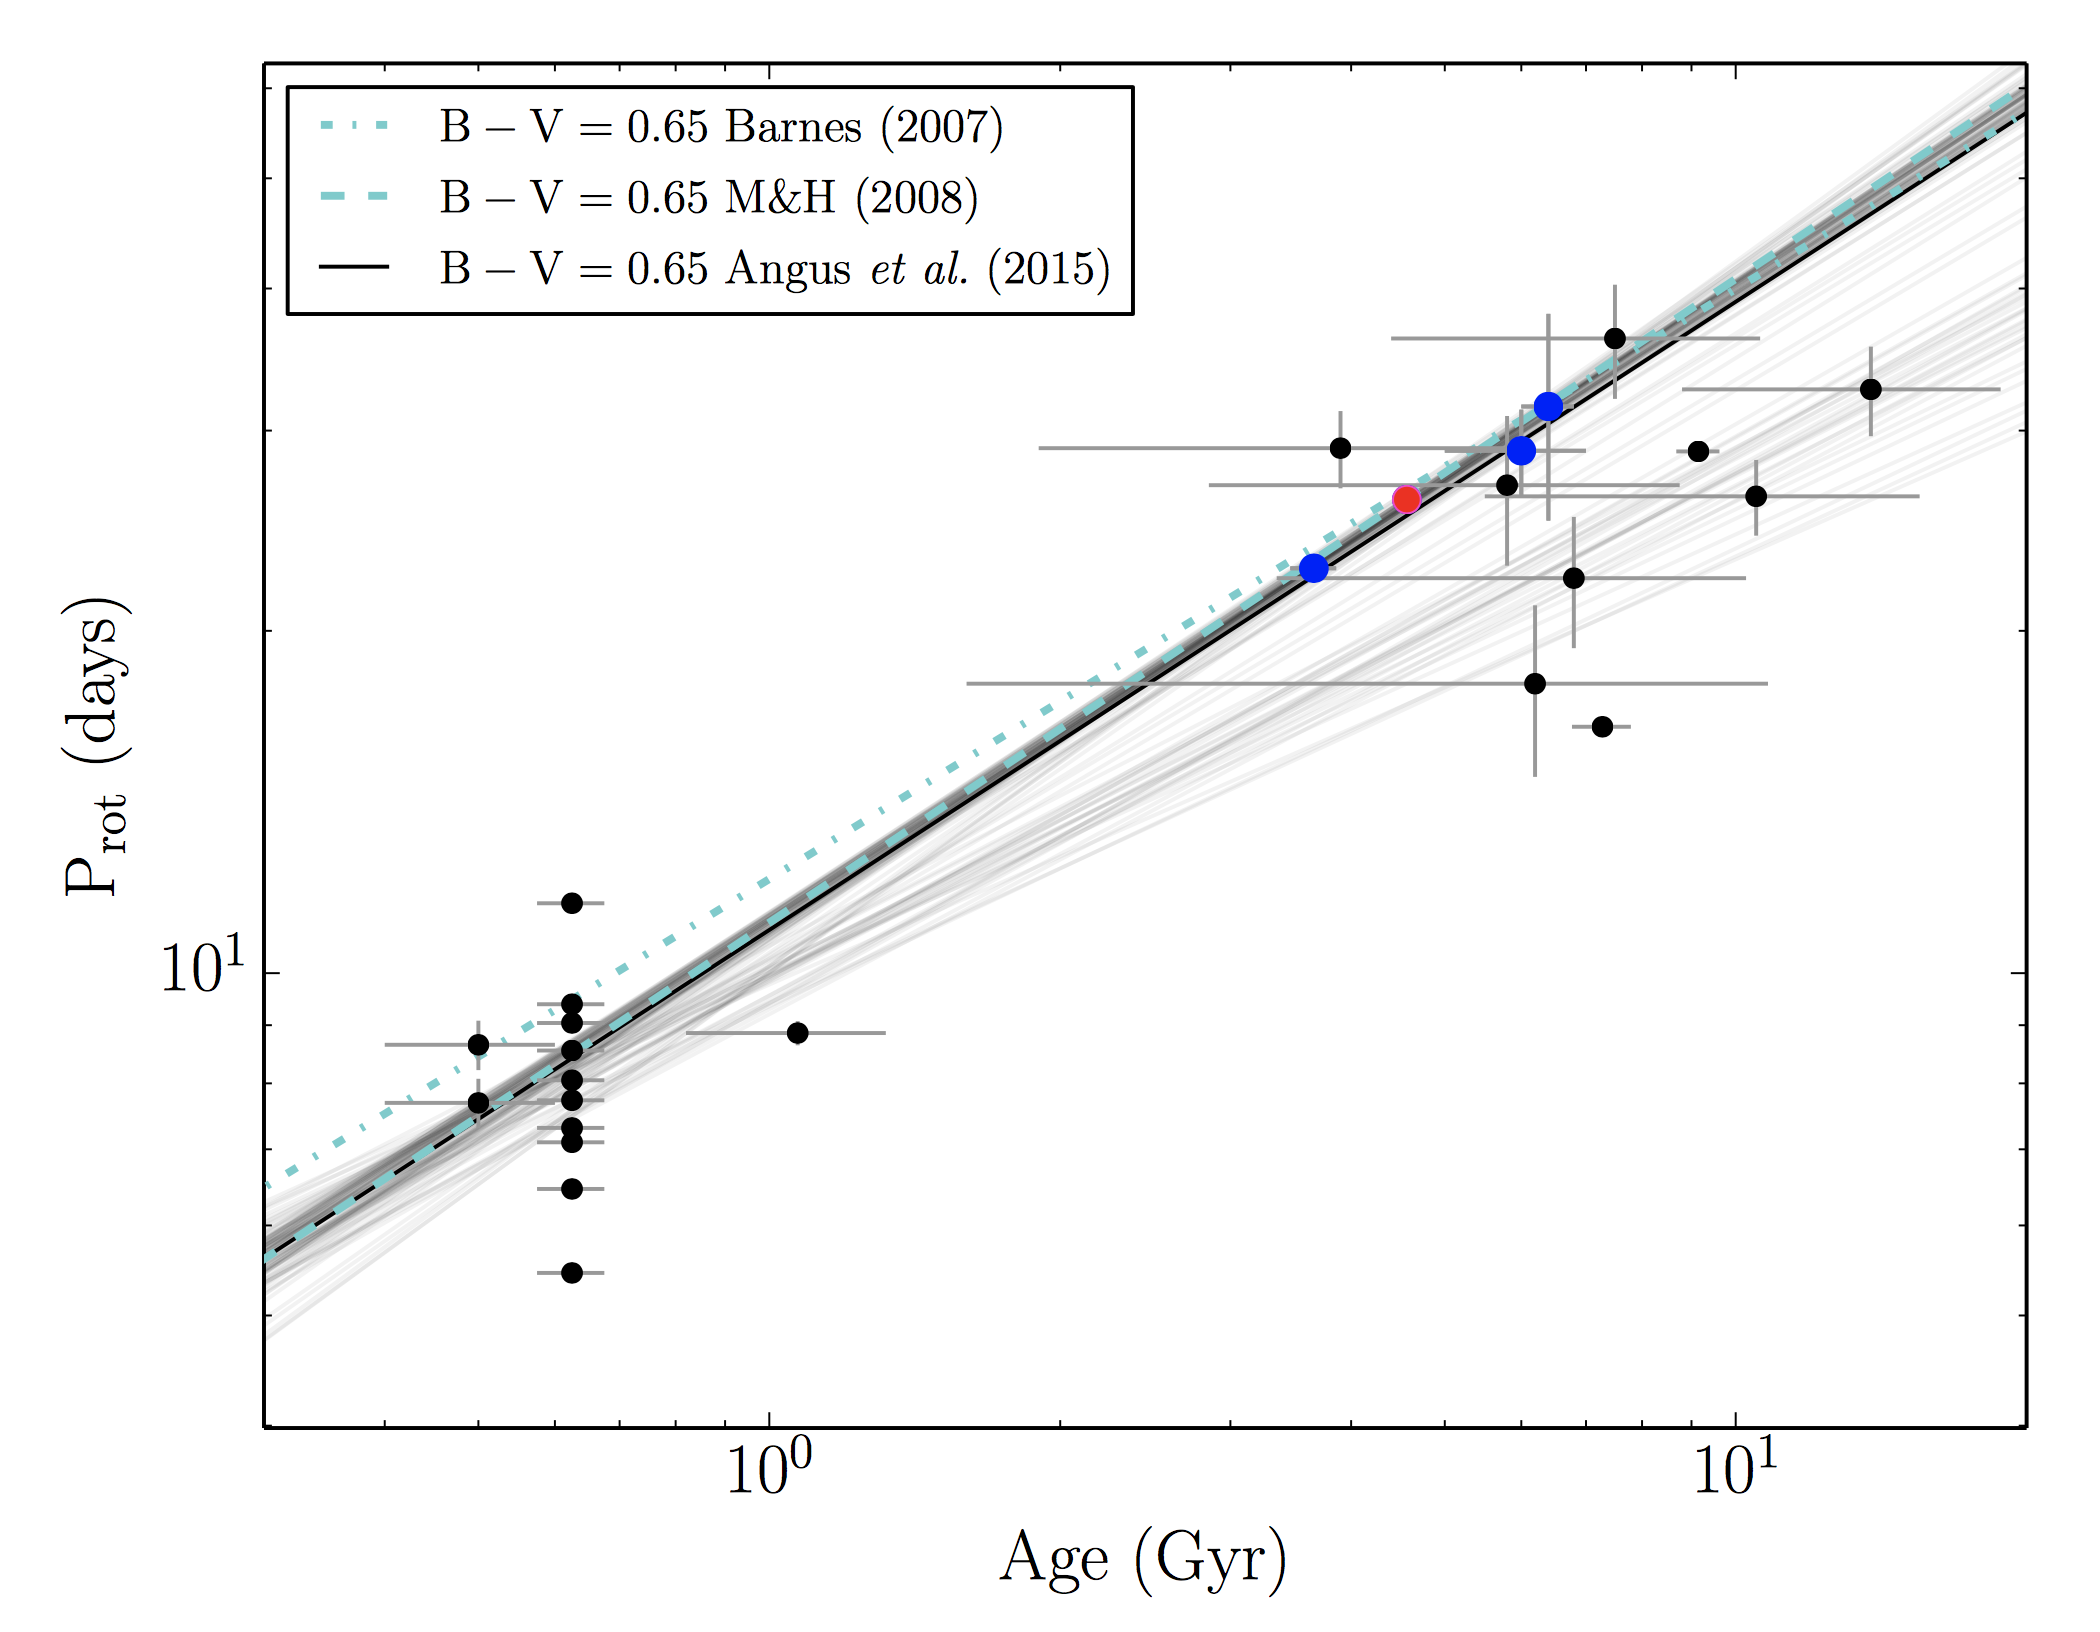
\includegraphics[width=4in]{angus2015_fig6.png}
\caption{Figure 6 from \citet{angus2015}, showing an improved gyrochronology relation calibrated using \Kepler asteroseismic targets (black dots) and the Sun (red dot), compared with other standard gyrochronology models (blue dashed and dotted lines).}
\label{fig:gyro}
\end{figure}


In Figure \ref{fig:gyro} we demonstrate the subtle differences between competing gyrochronology models for Solar mass stars. To increase the available sample of calibration sources available at Gyr ages, Co-I Angus has produced improved gyrochronology models using \Kepler asteroseismic targets \citep{angus2015}. Note: the additional calibration sources at Solar ages means the Angus model is not forced to exactly fit the Sun's rotation period, as other traditional models do. Unfortunately, asteroseismology cannot yet provide ages for stars with masses much lower than the Sun.  \Kepler rotation period samples have demonstrated that magnetic braking may become less efficient at older ages \citep{van-saders2016}.
The \citet{angus2015} gyrochronology study also found that cluster and asterosismic field star targets may not follow the same spin-down model, possibly indicating bias in the dynamical histories of these samples.  Additional calibration sources are desperately needed for stars older than the Sun, and for lower-mass dwarfs.







%%%%%%%%%
\subsection{Rotation Periods from \Kepler and K2}
Previous ground-based efforts to constrain stellar rotation periods for single, isolated field stars have resulted in few measurements. Detecting rotation from Doppler line broadening requires obtaining medium- to high-resolution spectroscopy of individual targets, and can be subject systematic effects such as from limb darkening approximations \citep{collins1995}. These observations also require time on larger aperture telescopes to reach fainter magnitudes needed to study rotation from low-mass field stars, or for studying the entire mass range within stellar clusters. Ground-based photometric wide-field surveys overcome many of the difficulties in gather large samples of field stars or entire stellar clusters. However, long duration monitoring with relatively high cadence and high photometric precision is required to detect the small amplitude and slowly varying flux modulations from starspots. These campaigns typically yielded rotation samples of hundreds to $\sim$1000 stars \citep[e.g.][]{hartman2010,hartman2011}


Space-based photometry surveys designed for exoplanet transit searches such as \Kepler \citep{borucki2010} have produced a revolution in stellar rotation studies. The original \Kepler mission produced light curves up to four years in duration with $\sim$100 ppm precision at 30-minute cadence for more than 200,000 stars. From this remarkable dataset, more than 30,000 unique stellar rotation periods have been measured using a variety of time series analysis techniques such as the Lomb-Scargle Periodogram \citep{reinhold2013} and the Autocorrelation Function \citep[][]{mcquillan2014}.
This bounty of rotation periods has also allowed the first ensemble investigations in to stellar surface differential rotation \citep[e.g.][]{reinhold2013}, revealed stars with near solid-body rotation \citep{davenport2015a}, and highlighted the many degeneracies in disentangling starspot evolution and differential rotation \citep{aigrain2015}.


After hardware failures made observations of the original field impossible, an extended \Kepler mission was designed to observe many fields with $\sim$3 month durations. The K2 mission has observed fields spaced along the ecliptic plane, ranging from low galactic latitudes that include multiple open clusters, to high galactic latitudes that include many older field stars \citep{howell2014}. The K2 fields also include several benchmark stellar clusters including the Solar-age M67, the Pleiades and Hyades, and M35. To date K2 has released data from 10 distinct campaigns (or fields), including more than 204,000 targets. An additional 4 campaigns are underway with $\sim$94,000 targets announced, and 2 campaigns pending scheduling. In total, the K2 sample may yield over 350,000 light curves, far exceeding the original \Kepler mission. Importantly, K2 data quality has been demonstrated to approach that of the original \Kepler mission \citep{luger2016}, and has been successfully used to measure rotation periods for select targets such as open cluster stars \citep[e.g.][]{douglas2017}.



{\bf K2 provides the ideal dataset to both extend the \Kepler studies of field star age distributions, and to amass a sample of better calibration sources for gyrochronology models.} The range of K2 fields positions within the Galaxy means the sample spans a much wider variety of stellar ages for more distant stars ($\gtrsim$1pc), and provides multiple opportunities to constrain the local star formation history for nearby stars. This makes the gyrochronology study of field stars with K2 an unique and valuable comparison to complimentary efforts in studying galactic archeology using chemical abundances, such as with APOGEE \citep{hayden2014}.
Producing rotation periods for these older stars, and the additional open clusters including the benchmark Solar age M67 available in the K2 data, will also lead to new gyrochronology relations, and to test the universality of the age--rotation--activity relation put into question by \citet{angus2015}.



%%%%%%%%%
\subsection{A Mysterious Period Bimodality}

One of the most remarkable results from the \Kepler rotation period catalog was the discovery of a bimodal period distribution among field stars by \citet{mcquillan2013}, and is shown in Figure \ref{fig:bimodal}a. While a separate sequence of rapid of rotation periods had been known in young stellar clusters due to lower-mass stars settling on to the angular momentum main sequence slower \citep[e.g.][]{barnes2007}, this new bimodality was detected from M dwarfs ($T_{eff}\lesssim4000$), and separated stars at a period of $\sim$20 days. Follow-up analysis of the \Kepler data by \citet{mcquillan2014} found the period bimodality extended to include K dwarfs. {\bf Recently, PI Davenport discovered this period bimodality extends throughout all masses in the \Kepler rotation sample for nearby stars, as shown in Figure \ref{fig:bimodal}b \citep{davenport2017}.} %By combining the \Kepler catalog with distance measurements from Gaia DR1 \citep{gaia_dr1}, contamination from subgiants .... -> put in later

\begin{figure}[!th]
\centering
\makebox[\textwidth][c]{ % sloppy hack to make figure slightly overflow
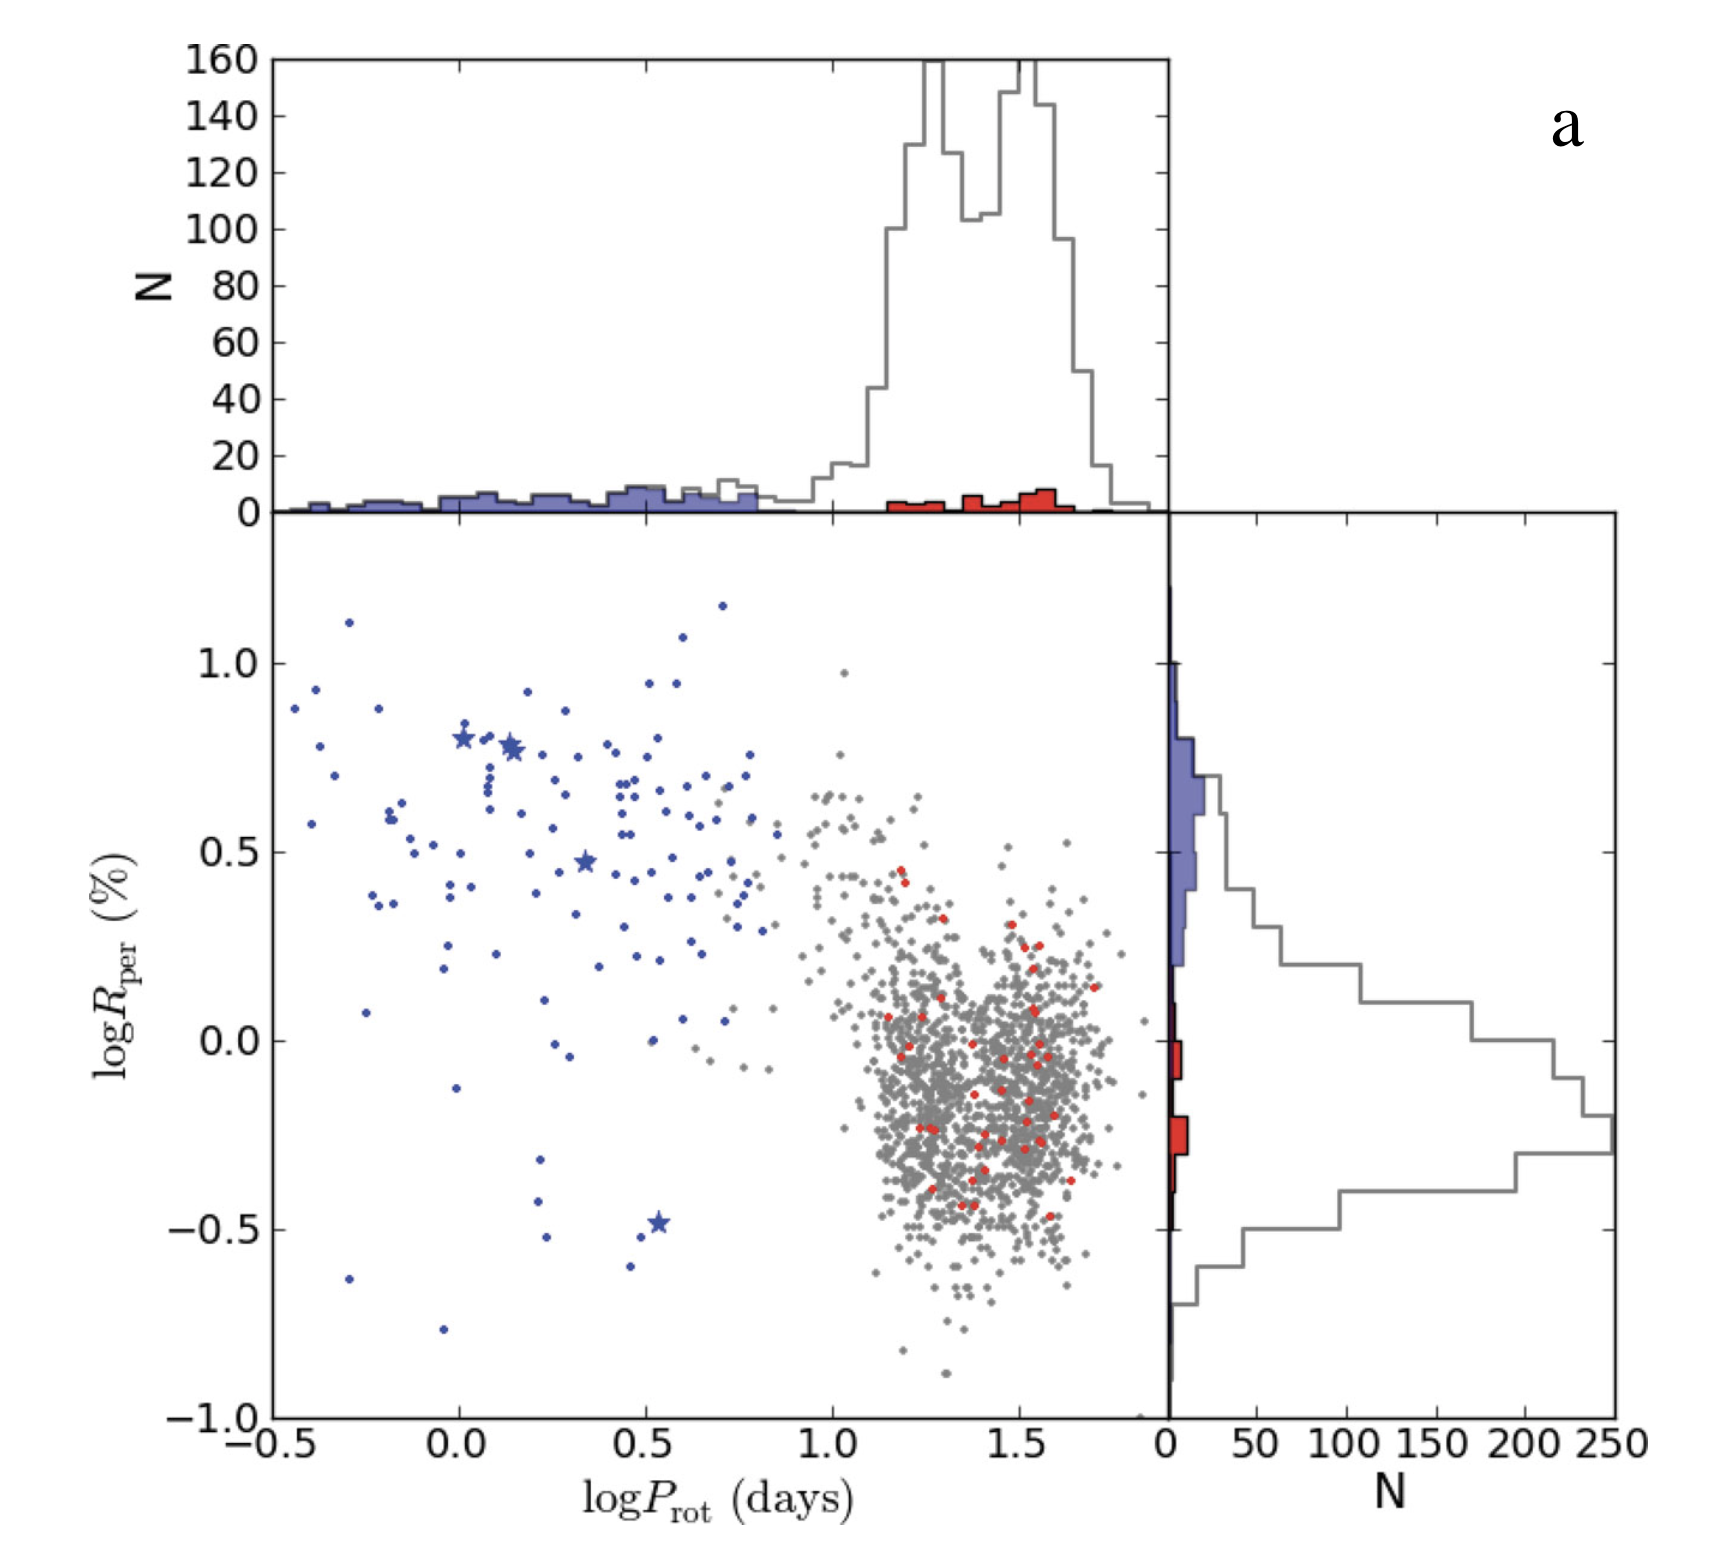
\includegraphics[width=3in]{mcquillan2013_fig9.png}
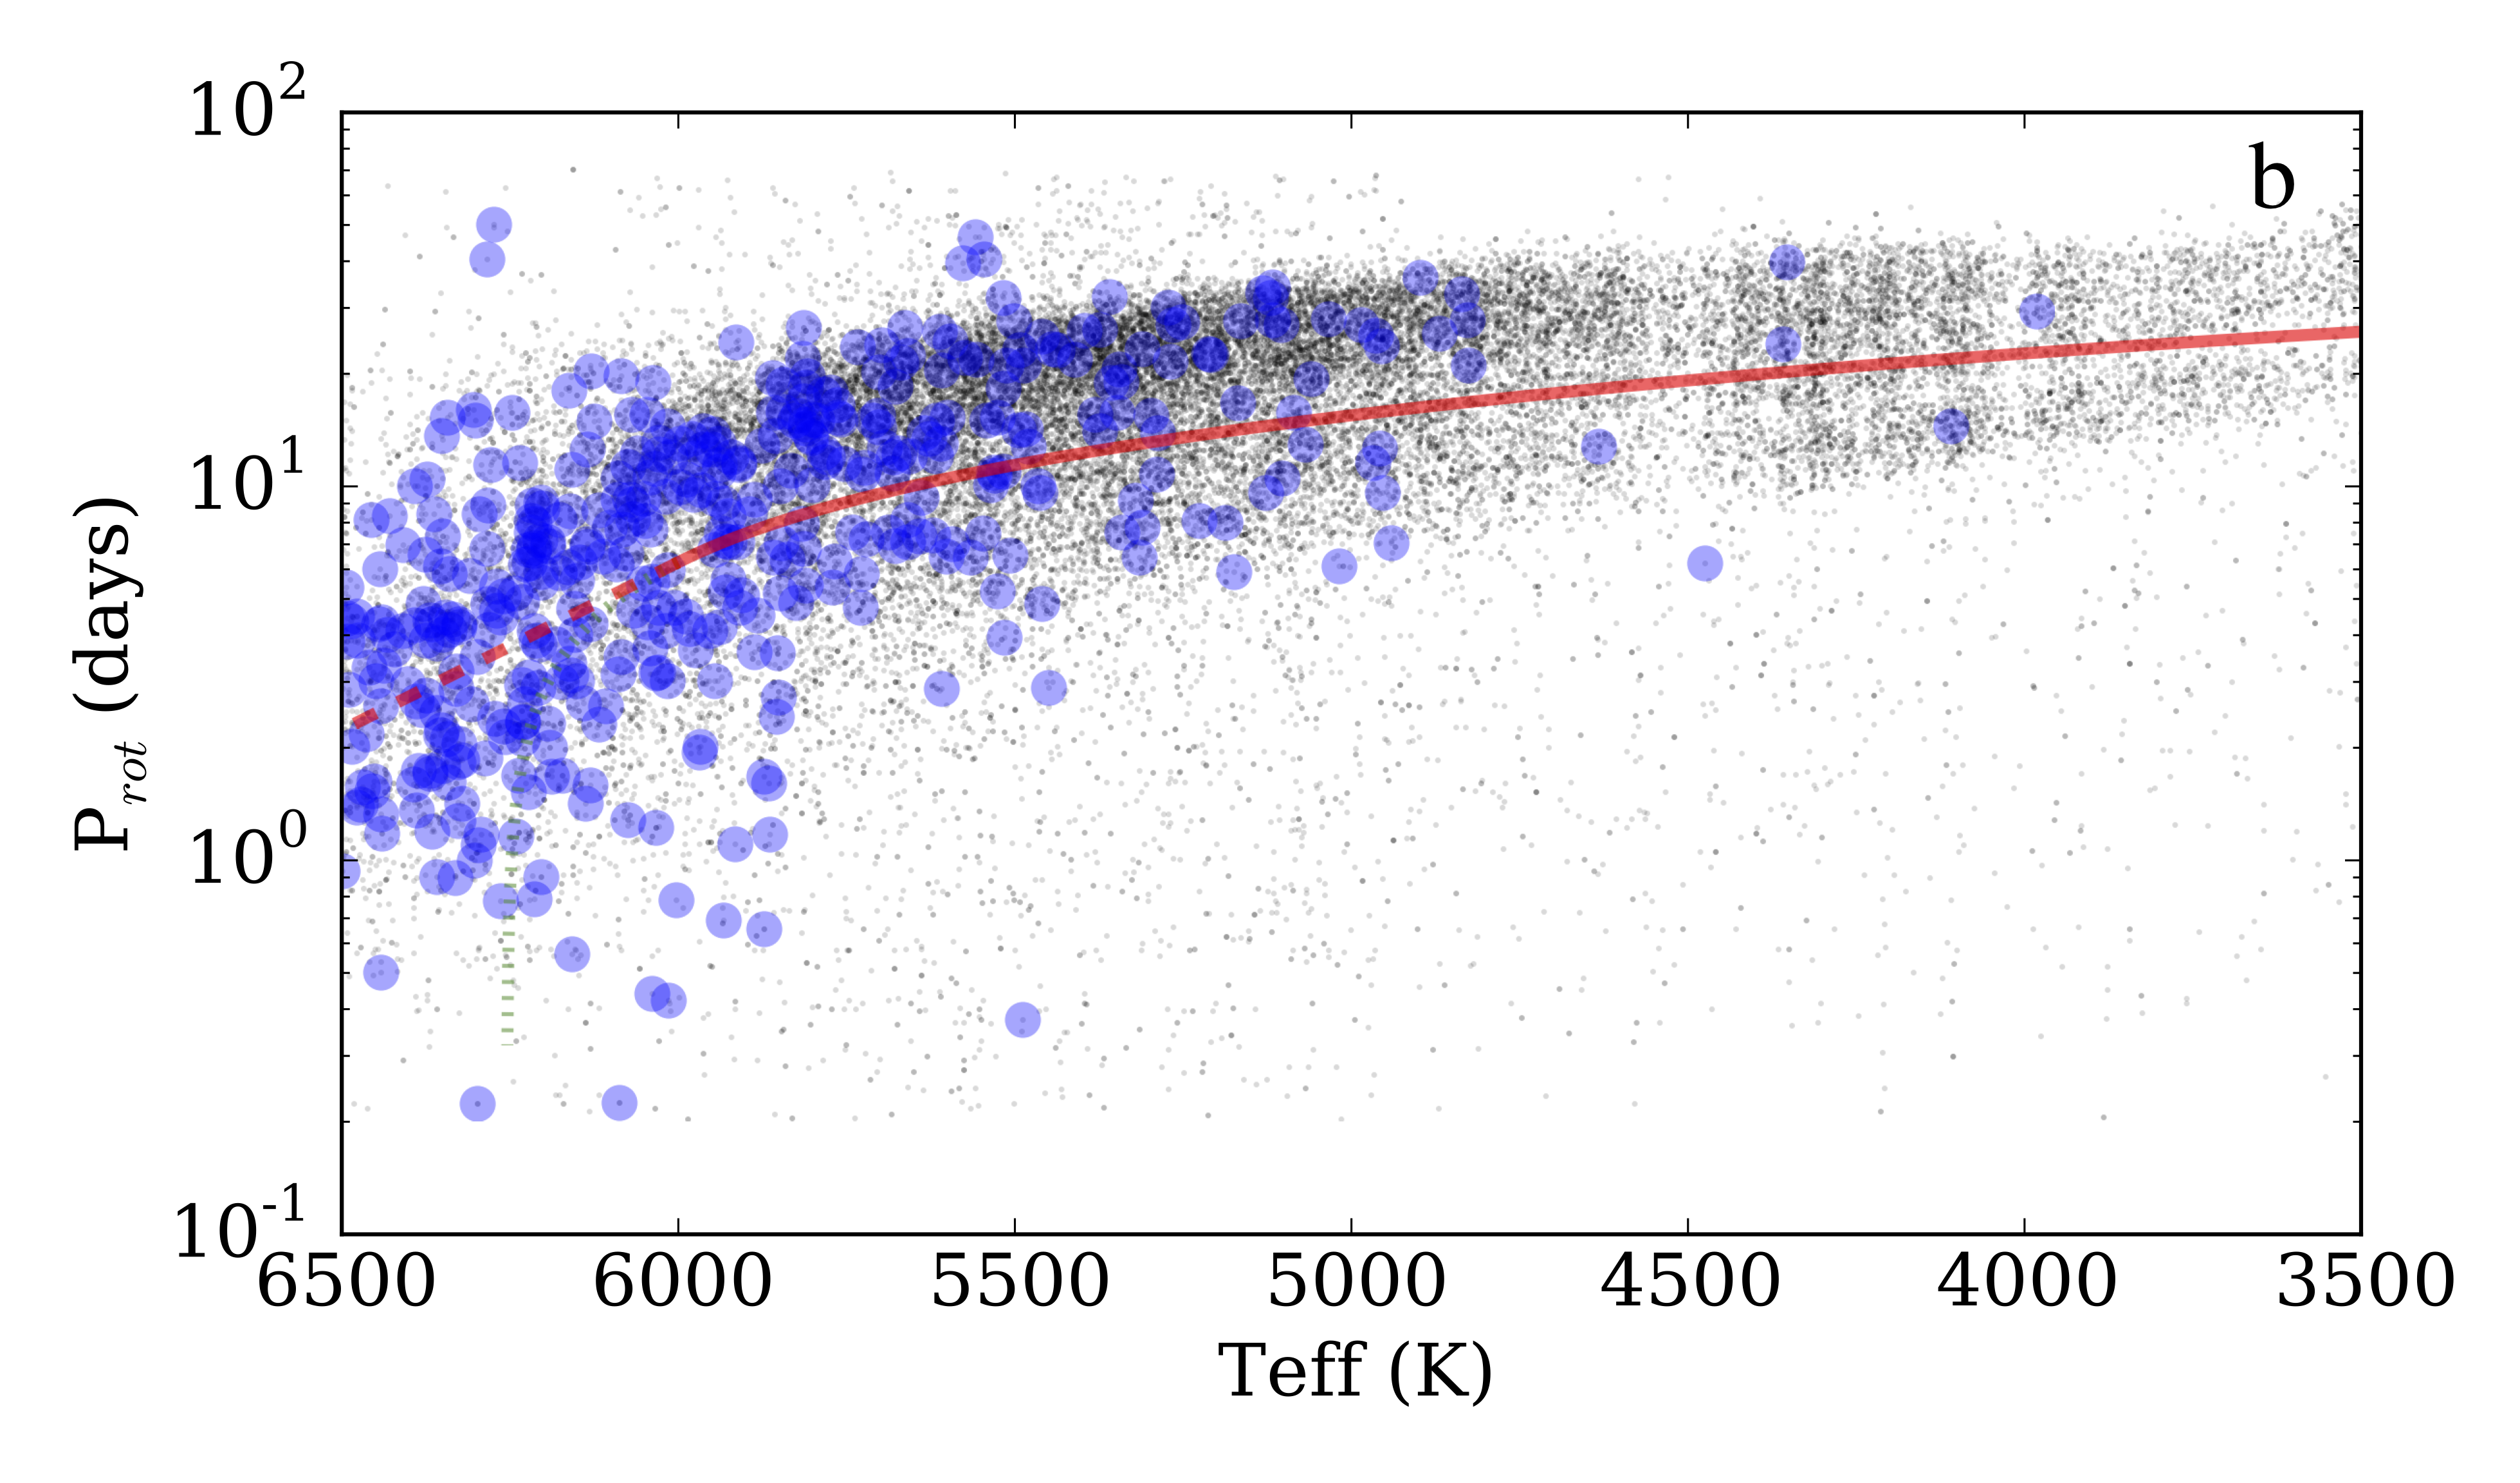
\includegraphics[width=4in]{davenport2016_fig3.png}
}
\caption{
Left -- Figure 9 from \citet{mcquillan2013}; the discovery of a bimodality in rotation periods from \Kepler M dwarfs (middle panel).
Right -- Figure 3 from \citet{davenport2017}, showing all \Kepler rotation periods from \citet{mcquillan2014} (black dots), and main sequence stars with Gaia DR1 distances (blue circles). The bimodality discovered for M dwarfs extends to nearby G and K stars, and straddles a 600 Myr ``gyrochrone'' (red line).
}
\label{fig:bimodal}
\end{figure}



%Explanations are either a break from single spin-down law (possibly from different initial periods, or some new physics maybe due to chemical abundances) or represents an age bimodality of local stars.
{\bf Two formation scenarios have been proposed to explain the observed period bimodality.} The first scenario, initially proposed by \citet{mcquillan2013}, is the rotation period distribution reflects the local star formation history, and thus the bimodality represents a drop in the star formation rate around 600 Myr ago. This model is supported by both the extension of the bimodality to earlier spectral types by \citet{davenport2017}, and also the tentative detection that the two rotation period populations have distinct proper motion distributions. However, such a variation in the star formation rate on short timescales has some tension with independent observational efforts to determine the local star formation history. While Color--Magnitude diagram inversions from Hipparcos have suggested a similarly short timescale variation in star formation of  $\sim$0.5 Gyr \citep{hernandez2000}, other studies find slower variations over several Gyr \citep[e.g.][]{cignoni2006}. Using white dwarf cooling models to infer the local formation history (``cosmochronology'') also supports higher star formation several Gyr ago, but can rarely achieve age resolution better than $\sim$1 Gyr due to small sample sizes \citep{tremblay2014}. The spatial extent of such coherent and localized variations in star formation history is unknown.

The second scenario to explain this feature is that the period bimodality occurs due to a previously unknown variation in the spin-down evolution for low-mass stars. In this scenario the star formation history would be continuous over the past $\sim$1 Gyr, and around 600 Myr stars would move quickly through the observed period minima due to this unknown phase transition or feedback mechanism. While this model is not currently predicted by angular momentum loss simulations, such rapid transition points in the angular momentum evolution are observed in young clusters. Stars move quickly from the rapidly rotating ``convective'' sequence (periods of $\lesssim1$ day) to the ``interface'' sequence (periods of several days) during the first few hundred Myr, with lower mass stars taking longer to make this transition as they settle onto the main sequence \citep{barnes2003}. 

{\bf The K2 rotation period sample provides the ideal dataset to test these two formation scenarios.} If the bimodality is due to an age distribution we would expect to only see the feature locally, and that it would disappear at further distances or along different lines of sight where small scale variations in the star formation history are less apparent. The kinematic separation between the two rotation period populations would be reinforced by supplemental measurements from the upcoming public Gaia data releases. However, if the bimodality is truly due to a transition point in the spin-down evolution at young ages, we would expect to find no little to no variation in this feature as seen in Figure \ref{fig:bimodal}b with galactic position or between K2 fields.

% Since this effect is seen only within 300pc so far (and only within Kepler data) due to sample properties, cannot be sure what spatial or compositional dependence this has, need a sample that spans a wider spatial area and more ages of stars
 
 
 


%%%%%%%%%%%%%%%%%%%
\section{Proposed Research}
%%%%%%%%%
\subsection{Measuring Rotation periods}
We propose the first systematic study of stellar rotation periods from the K2
data. This will include the nearly 300,000 light curves from Campaigns 0-14.
%This includes data for multiple stellar clusters that were taken as part of
%the Guest Observer program.
%\racomment{
%I'm not sure we want to get into measuring rotation periods for
%stars in the cluster superstamps. Besides, there are other people working on
%this. I think we should stick to the regular K2 targets.
%}
%JRAD: I totally agree

Part of our study will be to assess the qualities of the various data
reduction pipelines available for K2 light curves.
Each detrending algorithm uses a slightly different approach and will almost
certainly provide light curves that differ enough to produce a number of
discrepant rotation periods.
We will compare the performance of three pipelines in particular: the
\citet{Vanderburg2015} light curves, the {\tt everest} \citet{luger2016} light
curves, and the \ktwosc\ \citet{aigrain2016} light curves.
By visually examining the light curves and Lomb-Scargle periodograms of a
number of targets in common between the detrending methods, we will ascertain
which pipeline best preserves signal on long timescales.
% The \ktwosc\ pipeline removes instrumental systematics using a non-parametric
% approach: a Gaussian process is used to model the instrumental systematics,
% astrophysical variability and white noise in each light curve.
All three of these pipelines are optimized for planet search, however the
\citet{aigrain2016} light curves are designed to preserve stellar variability
as much as possible.
We expect to find that these light curves preserve rotation signals on the
longest timescales.


Once establishing the best detrending method for preserving stellar
variability, we will download all the available light curves and, if
necessary, run the pipeline on any outstanding targets.
We will also produce and examine periodograms using the
systematics-insensitive periodogram (SIP) \citep{angus2015}.
This method simultaneously fits light curves with a sinusoid and a noise
model constructed from 150 principle components derived from a PCA of the
entire set of \ktwo\ light curves for a given campaign.
Although developed for asteroseismology, this algorithm may also be applicable
to rotation period analysis, however at the longer timescales of variation
produced by stellar rotation, it is likely that the results will suffer
from overfitting.

We will use a combination of Lomb-Scargle and autocorrelation function
techniques to produce a quick catalogue for early analysis.
Although both of these methods are sensitive to noise and can produce spurious
rotation period measurements, there relative speed will allow us to rapidly
begin initial analysis of the results.
We will then apply a procedure for obtaining more accurate and precise
rotation periods using probabilistic inference.
Co-I Angus recently developed a method for rotation period inference using a
Gaussian Process (GP) to model the light curve in the time-domain, rather than
extracting periodic signals in the frequency domain \citet{angus2016c}. 
% Is this IAU reference correct, or do you have a paper?%\citet{Angus2017}.
This GP method produces slightly more precise and accurate rotation periods
with more representative uncertainties than Lomb-Scargle and autocorrelation
methods.
The disadvantage of this GP regression based method is that it can be
computationally expensive.
However, with the recently developed method for fast Gaussian process
inference, {\tt celerite} \citep{foreman-mackey2017}, even performing MCMC
with the thousands of data points in a \ktwo\ light curve may only take a few
minutes.
The advantage of computing probabilistic rotation periods is that one can
bypass the need to calculate a rotation period at all and simply infer the
parameters of stellar populations directly from the light curves themselves.
In other words, one can perform hierarchical inference more easily.
This may be a level of sophistication that is above and beyond our science
goals but it is worth noting that we could take this approach if the data and
scientific question warranted it.

Wherever possible we will mask out discontinuous astrophysical signals, such as
eclipsing binaries, planet transit or flares that may distort the rotation
period signal.
We will make use of exoplanet and binary catalogs to identify planet transits
and eclipses.
We will apply the flare detection algorithm {\tt appaloosa}, built by PI Davenport, 
to identify and remove flares.
It may still be necessary to apply a low-pass filter to the data in order to
remove high frequency features that we miss.
Fortunately, most of the stellar rotation signals of interest for this study
have timescales longer than around a day and will be relatively unaffected by
a low-pass filtering algorithm.

The \Kepler rotation period catalog from \citet{mcquillan2014} found a yield
of $\sim25\%$ of stars had measurable rotation periods using the
Autocorrelation Function. From our sample of nearly 300,000 available K2 targets, we
expect to recover over 70,000 new periods, bringing the total
\Kepler/K2 sample to $\sim$100,000 stars with measured rotation periods.

We have already measured a number of \ktwo\ rotation periods using an
autocorrelation function approach.

% \begin{figure}[!th]
% \centering
% 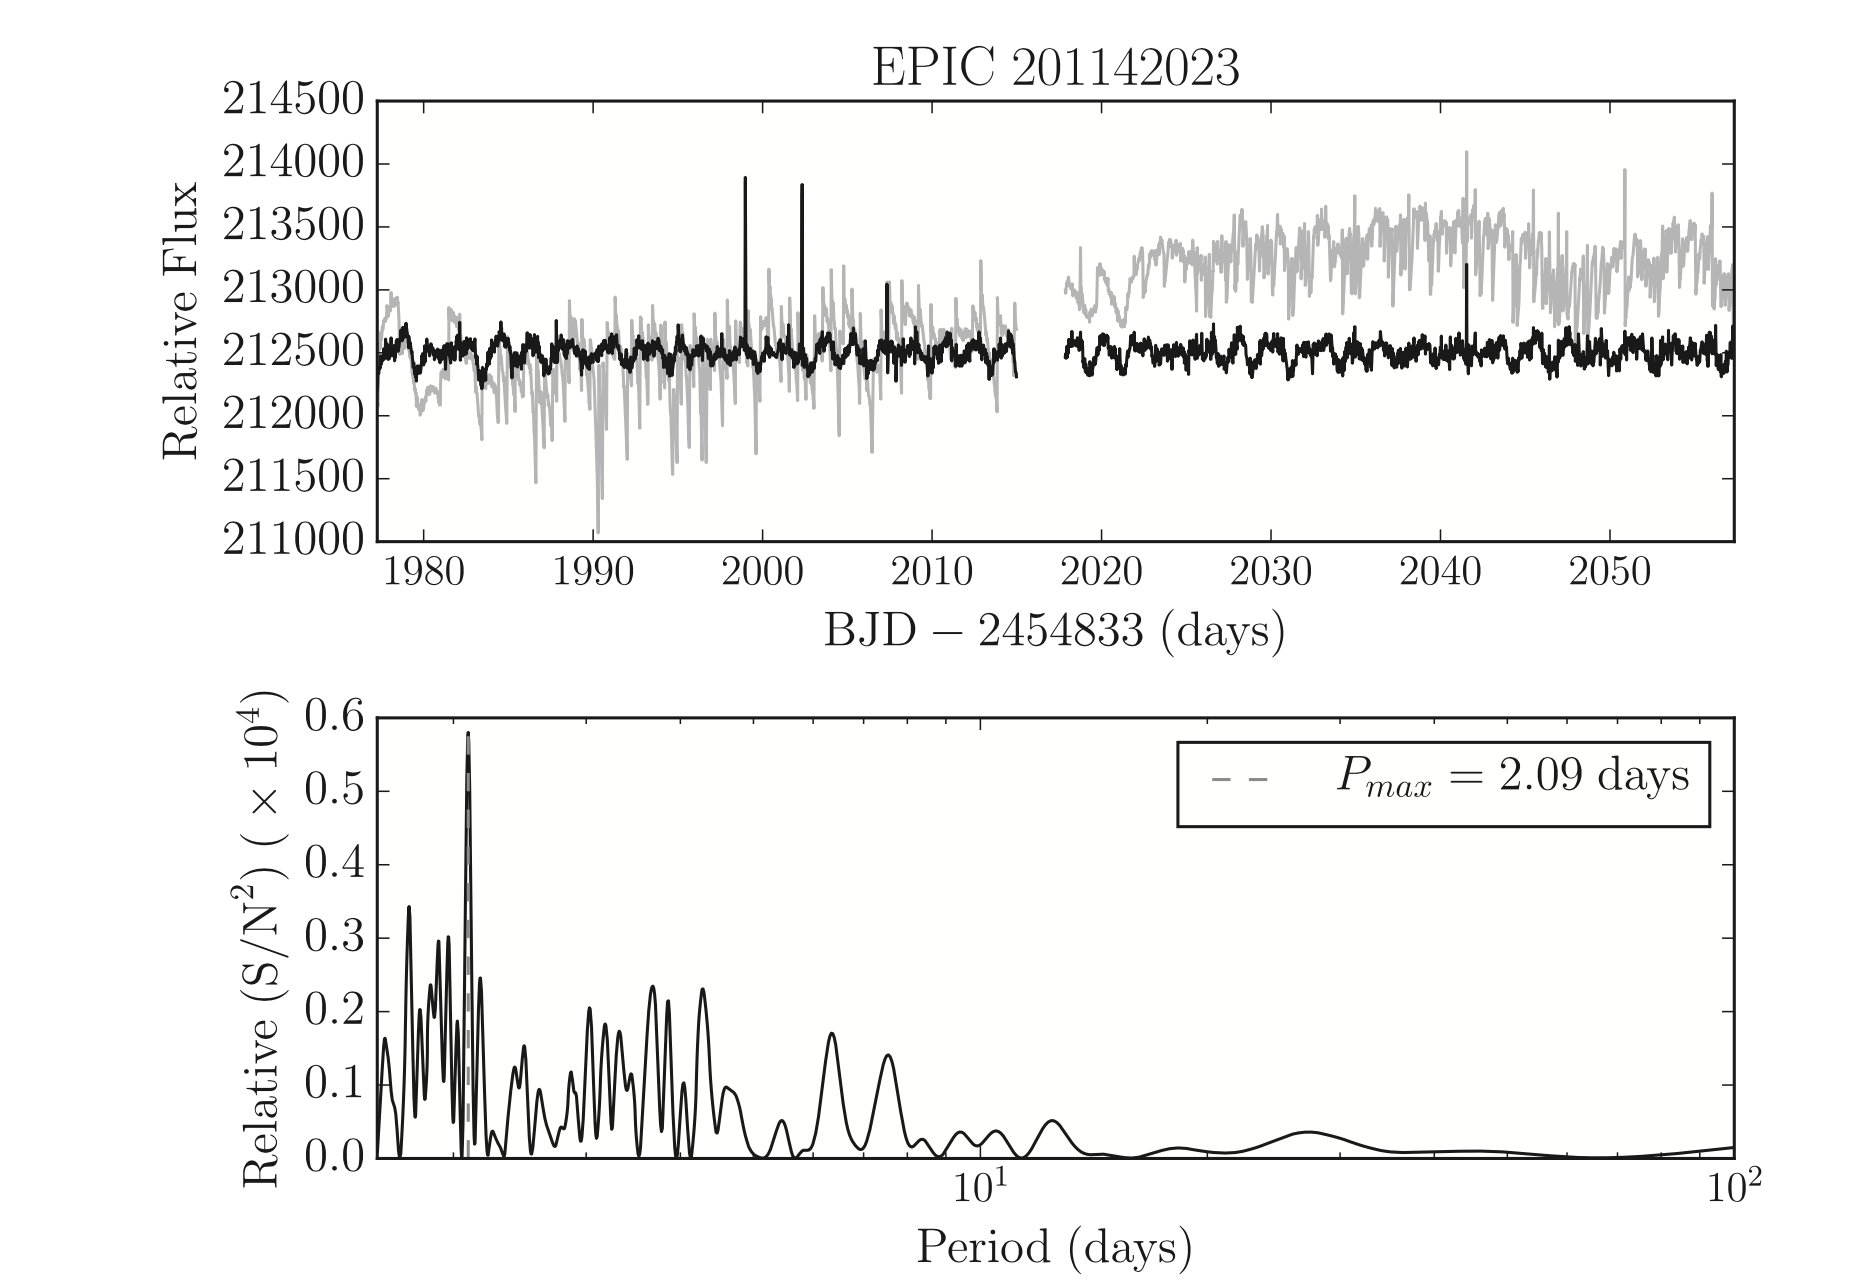
\includegraphics[width=4in]{angus2016_fig6.png}
% \caption{
% figure 6 from \citet{angus2016}, showing the processing of the light curve and resulting SIPeriodogram. more simple methods give erroneous periods for this object of either 3 days via ACF, or 59 days via normal Lomb-Scargle methods.
% }
% \label{fig:sip}
% \end{figure}





%%%%%%%%%
\subsection{Exploring the Period Bimodality}
by combining our sample with the distances provided in the forthcoming Gaia DR2 catalog, we will be able to extend the methodology of \citet{davenport2017} to filter our subgiants and binary stars for our entire sample.

we then can make 3d exploration of period distribution, to see if the bimodality exists for all field stars near the sun.

the big goal here is to decide which explanation is correct!

\begin{figure}[!th]
\centering
\makebox[\textwidth][c]{ % sloppy hack to make figure slightly overflow
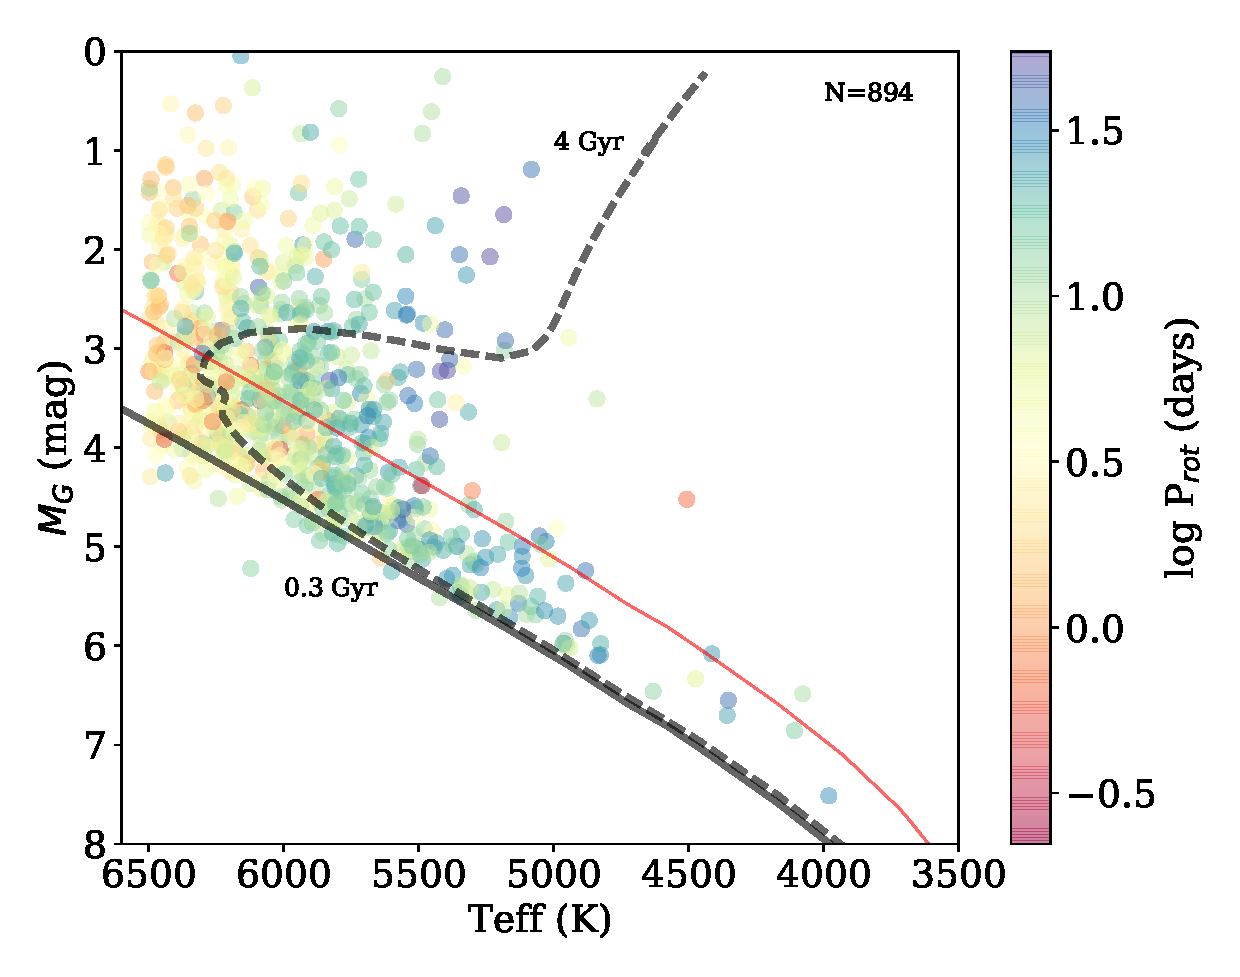
\includegraphics[width=3.5in]{davenport2016_fig2}
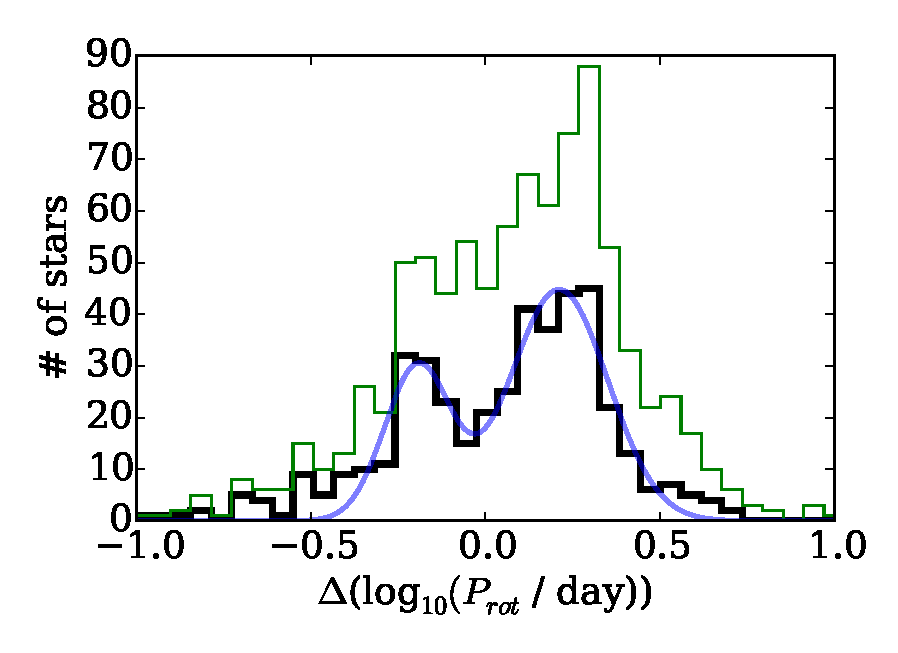
\includegraphics[width=3in]{davenport2016_fig4}
}
\caption{Left -- Figure 2 from \citet{davenport2017}, showing the absolute Gaia magnitude versus temperature for \Kepler stars with known rotation periods in the Gaia DR1 catalog. Sub-giant stars can be separated from main sequence targets using isochrone models (black solid \& dashed lines). Right -- Figure 4 from \citet{davenport2017}, showing the rotation period distribution relative to a 600 Myr ``gyrochrone'' before (green line) and after (black line) filtering our sub-giants. The bimodal distribution is apparent, and fit with a 2-Gaussian model (blue line).}
\label{fig:cmd}
\end{figure}

data from the Gaia mission \citep{perryman2001}
gaia DR1 \citep{gaia_dr1}



%%%%%%%%%
\subsection{Mapping Ages in each Field}

%Demonstration figure?
\begin{figure}[!th]
\centering
%\includegraphics[width=3.5in]{}
\fbox{\rule{3in}{0pt}\rule[-0.5ex]{0pt}{24ex}}
\caption{
DEMONSTRATION FIGURE OF CHRONOMETER? 
}
\label{fig:chrono}
\end{figure}



our catalog of rotation periods from K2, combined with existing catalogs from Kepler, we will have the largest set of rotation periods ever to use for population analysis. using new technique being developed by Ruth (Chronometer) we will have improved age estimate for every star based on single rotation values. then we combine this to get age distribution within each K2 field.


%discussion of improved gyrochronology calibration?

this is partially an extension of the period bimodality work (if it's an age effect), but to create a detailed map of the ages of these field stars at a range of galactic latitudes in the 17 pencil-beams available from K2. combining with the periods from Kepler, will be even better. ultimately we'd like to compare to the age distributions in simulations of these fields from TRILEGAL, and from other age indicators (asteroseismology, flare ages, etc)



%%%%%%%%%%%%%%%%%%%
\section{Team Qualifications}
PI Davenport has used \Kepler to conduct the largest survey to-date of stellar activity from flares, as well as multiple investigations of starspots and their evolution with time using \Kepler data. From these studies, Davenport has developed an age model for flare activity that will be directly comparable to the ages and starspot amplitudes derived from this study. He also recently discovered the rotation period bimodality first noted with \Kepler M dwarfs by \citet{mcquillan2013} extends to G and K dwarf stars \citep{davenport2017}.
Davenport previously collaborated on NASA ADP grant NNX09AC77G to characterize NIR variability using the 2MASS Calibration Scan Point Source Working Database \citep{davenport2012,davenport2015a}.
He has mentored numerous students on projects using \Kepler data, resulting in student-led publications such as the flare activity of a unique M dwarf binary system GJ 1245AB \citep{lurie2015}, and exploring the poorly understood origins of wide binary stars through stellar rotation (R. Clarke in prep). He will manage the overall project, detect and remove short period variability from flares in the light curves, and lead the investigation and publication on the nature of the bimodal period distribution.

Co-I Angus is an expert in the extraction of periodic signals from \Kepler data using Gaussian Processes \citep{angus2016c} and other cutting-edge statistical techniques. She is the author of tools for generating Systematics-Insensitive Periodograms for both \Kepler and K2 data \citep{angus2016}, as well as new gyrochronology calibrations using \Kepler asteroseismic targets \citep{angus2015}. She will lead the effort to measure and publish rotation periods for all K2 sources, and guide students in measuring ages for field stars.

Covey

Kipping

Agueros

%%%%%%%%%%%%%%%%%%%
\section{Relevance to NASA Programs}
history of MWY, age of planet systems, TESS



%%%%%%%%%%%%%%%%%%%
\section{Plan of Work}
{\bf Year 1:} process all rotation period data
\\
{\bf Year 2:} write papers



\clearpage
%\pagestyle{empty}

\bibliography{/Users/james/Dropbox/references}


\end{document}

